\chapter{Tutorial}
\label{tutorial}

This tutorial should provide the user with a tour through the most important functionalities of RODIN, so that he gets a understanding of how the program works.

The tutorial doesn't contain all the knowledge that you require.  Instead, it touches upon every concept - from installation to set theory to modeling and refinement - and helps you to find gaps in your knowledge.

Before we build a first model, we will cover some basic math.

\section{Theory to Get You Started}
\label{tutorial_theory}

\tick{\textbf{Goals:} The focus of this section is to briefly cover all the required theory, and to provide pointers for further reading.  Specifically, this includes Propositional Calculus, First Order Predicate Calculus, Set Theory and Arithmetic}

\paragraph{See Also:}
\begin{itemize}
\item Mathematical Notation Slides \url{files/sld_mth1.pdf}
\end{itemize}


\section{Getting around Rodin}
\label{tutorial_2}

\tick{\textbf{Goals:} In this section, we cover installation, the basic features of an Eclipse application, and the Rodin-specific GUI elements.}


\section{Example 1: A Trafficlight Controller}
\label{tutorial_3}

\tick{\textbf{Goals:} The focus of this section is modeling.  You will learn how to model a simple system (a traffic light controller).  We will use this example to introduce the concept of refinement (\ref{refinement}).  The proofs in this section should all be discharged automatically. }

The following picture visualizes the problem we are going to solve:

\begin{center}
	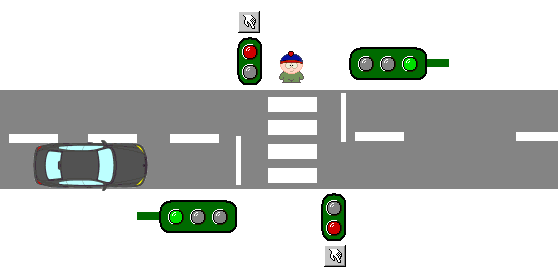
\includegraphics[width=0.9\textwidth]{img/tutorial/trafficlight.png}
\end{center}

The objective is to design the software for a controller that switches the trafficlights and that reacts to pedestrian requests to cross the street.

We tackle the problem in multiple steps:

\begin{enumerate}
	\item We will abstract the problem and develop a refinement plan (\ref{tutorial_tl_problem_abstraction})
	\item We will implement the initial model (\ref{tutorial_tl_initial_model})
	\item We will perform Data Refinement (\ref{data_refinement})
\end{enumerate}

\subsection{Problem Abstraction}
\label{tutorial_tl_problem_abstraction}

\subsection{Initial Model}
\label{tutorial_tl_initial_model}

\subsubsection{Project Setup}

First create a new Event-B Project \textsf{File $\rangle$ New $\rangle$ Event-B Project}.  Give the project the name \texttt{trafficlight}.

Next, create a Machine.  Right-click the newly created project and select \textsf{New $\rangle$ Event-B Component}.  Call the component \texttt{mac0}.

\info{A good naming convention can save a lot of work.  We have a recommended naming convention (\ref{naming_convention})}

\subsubsection{System State}

We will now add the variables that store the traffic light value as a boolean.

\tick{A new variable requires three elements: The variable itself, the typing invariant and the initialization.  But typically, we'd also add events that change the state.  And there may be further invariants constraining the state.}



\pencil{
\begin{description}
\VARIABLES
	\begin{description}
		\Item{ cars\_go }
	\end{description}
\INVARIANTS
	\begin{description}
		\nItemX{ inv1 }{ cars\_go \in  BOOL }
	\end{description}
\EVENTS
	\INITIALISATION
		\begin{description}
		\BeginAct
			\begin{description}
			\nItemX{ act1 }{ cars\_go :=  FALSE }
			\end{description}
		\EndAct
		\end{description}
\END
\end{description}
}


\info{There are various ways to accelerate the creation of variables.  The structural editor has a wizard for this purpose.}

\pencil{
\begin{description}
\MACHINE{mac0}
\VARIABLES
	\begin{description}
		\Item{ cars\_go }
		\Item{ peds\_go }
	\end{description}
\INVARIANTS
	\begin{description}
		\nItemX{ inv1 }{ cars\_go \in  BOOL }
		\nItemX{ inv2 }{ peds\_go \in  BOOL }
		\nItemX{ inv3 }{ \lnot  (cars\_go = TRUE \land  peds\_go = TRUE) }
	\end{description}
\EVENTS
	\INITIALISATION
		\begin{description}
		\BeginAct
			\begin{description}
			\nItemX{ act1 }{ cars\_go :=  FALSE }
			\nItemX{ act2 }{ peds\_go :=  FALSE }
			\end{description}
		\EndAct
		\end{description}
	\EVT {cars\_light}
		\begin{description}
		\AnyPrm
			\begin{description}
			\ItemX{ new\_value }
			\end{description}
		\WhereGrd
			\begin{description}
			\nItemX{ grd1 }{ \lnot  (new\_value = TRUE \land  peds\_go = TRUE) }
			\end{description}
		\ThenAct
			\begin{description}
			\nItemX{ act1 }{ cars\_go :=  new\_value }
			\end{description}
		\EndAct
		\end{description}
	\EVT {peds\_light}
		\begin{description}
		\AnyPrm
			\begin{description}
			\ItemX{ new\_value }
			\end{description}
		\WhereGrd
			\begin{description}
			\nItemX{ grd1 }{ \lnot  (cars\_go = TRUE \land  new\_value = TRUE) }
			\end{description}
		\ThenAct
			\begin{description}
			\nItemX{ act1 }{ peds\_go :=  new\_value }
			\end{description}
		\EndAct
		\end{description}
\END
\end{description}
}

\subsection{Data Refinement: Introduce Trafficlight Colors}
\label{tutorial_tl_data_refinement}


- simple proofs
- refinement

\section{Excurs: Data Structures}
\label{tutorial_4}

\section{Excurs: Proofing}
\label{tutorial_5}

\section{A more complex Example}


